\documentclass{nthuthesis}

% === Define Package
\usepackage{times}
\usepackage{newtxmath}  % for the Times New Roman font for equation
\usepackage{verbatim}
\usepackage{color}
\usepackage{url}
\usepackage{graphicx}
\usepackage{array}
\usepackage{wallpaper}
\usepackage{cite}
\usepackage{caption}
\usepackage{subcaption}
\usepackage{siunitx}
\usepackage{physics}
\usepackage{booktabs}
\usepackage{multirow}
\usepackage{makecell}
\usepackage{hhline}
\usepackage{rotating}
\usepackage{amsmath}
\let\Bbbk\relax % redefined in newtxmath.sty, combine with newtxmath.
\usepackage{tikz}
\usepackage{floatrow}
\usepackage{listings} % for highlight code
\usepackage{titlesec}
\usepackage{bm}
\usepackage{amssymb}
\usepackage{mathrsfs}
\usepackage{ragged2e}
\usepackage{indentfirst}
\usepackage{emptypage} % for twoside empty page after chapter if the page is not start from odd number
\usepackage{titletoc}
\usepackage{zhnumber} % for Chinese number
\usepackage{svg}
\usepackage{notoccite} % PREVENTS CITES IN CAPTIONS FROM MISNUMBERING YOUR REFERENCES

% for algorithm
\usepackage[algochapter,ruled,linesnumbered]{algorithm2e}

% To customize item and enumerate
\usepackage{enumitem}

% to allow equation break the page
\allowdisplaybreaks

% \usepackage[hidelinks]{hyperref} % hyperlink for everything

% setting for cleveref
\usepackage{cleveref}
\crefformat{figure}{圖~#2#1#3~}
\crefformat{table}{表~#2#1#3~}
\crefformat{equation}{~(#2#1#3)~式}
\crefformat{algorithm}{演算法~#2#1#3~(Algorithm~#2#1#3)~}
\crefformat{chapter}{第#2\zhnumber{#1}#3章}
\crefformat{section}{~#2#1#3~節}
\crefformat{subsection}{~#2#1#3~小節}
\crefformat{appendix}{附錄~#2#1#3~}

\floatsetup[table]{capposition=top}

\makeatletter

% Reinsert missing \algbackskip
\def\algbackskip{\hskip-\ALG@thistlm}

\providecommand\add@text{}
\newcommand\tagaddtext[1]{%
  \gdef\add@text{#1\gdef\add@text{}}}% 
  
\renewcommand\tagform@[1]{%
  \maketag@@@{\llap{\add@text\quad}(\ignorespaces#1\unskip\@@italiccorr)}%
}

\makeatother



% declare the path(s) where your graphic files are
\graphicspath{{./figsrc/}}
% and their extensions so you won't have to specify these with
% every instance of \includegraphics
% \DeclareGraphicsExtensions{.pdf,.jpeg,.png}

% Using the tex-text mapping for ligatures etc.
\defaultfontfeatures{Mapping=tex-text}

% Set the default fonts

% English font
% Note: please refer to 'fc-list :outline -f "%{family}\n"' for choosing a valid font name
\usepackage{fontspec}
%\setmainfont{Times New Roman.ttf}
\setmainfont{Times New Roman}

% Chinese font
% Note: please refer to 'fc-list :outline -f "%{family}\n"' for choosing a valid font name
\setCJKmainfont[AutoFakeBold=3,AutoFakeSlant=.4]{kaiu.ttf}
\setCJKmonofont[AutoFakeBold=3,AutoFakeSlant=.4]{kaiu.ttf}
\defaultCJKfontfeatures{AutoFakeBold=6,AutoFakeSlant=.4}

\CenterWallPaper{0.25}{nthu_logo_85.png}


% Title Setting
\titleformat{\chapter}
  {\Large\bfseries\centering}
  {第\,\zhnumber{\thechapter}\,章}{1em}{\Large}

\titleformat{\section}
  {\large\bfseries}
  {\thesection}{1em}{\large}

\titleformat{\subsection}
  {\normalsize\bfseries}
  {\thesubsection}{1em}{\normalsize}

\titlespacing*{\chapter}{0pt}{-1.3cm}{0pt}
\titlespacing*{\section}{0pt}{14pt}{0pt}
\titlespacing*{\subsection}{0pt}{14pt}{0pt}
\titlespacing*{\subsubsection}{0pt}{0pt}{0pt}

% TOC setting
\titlecontents{chapter}% <section-type>
  [0pt]% <left>
  {}% <above-code>
  {\bfseries 第\zhnumber{\thecontentslabel}章\quad}% <numbered-entry-format>
  {\bfseries}% <numberless-entry-format>
  {\bfseries\hfill\contentspage}% <filler-page-format>

% 將英文標示改為中文
\renewcommand{\contentsname}{目錄}
\renewcommand{\listfigurename}{圖目錄}
\renewcommand{\listtablename}{表目錄}
\renewcommand{\figurename}{圖}
\renewcommand{\tablename}{表}
\captionsetup[figure]{labelsep=space}
\captionsetup[subfigure]{font=normalsize}
\captionsetup[table]{labelsep=space}

% 行距設定
\linespread{2.0}

% Your information goes here
% author: Tz-Huan Huang [http://www.csie.ntu.edu.tw/~tzhuan]

% ----------------------------------------------------------------------------
% "THE CHOCOLATE-WARE LICENSE":
% Tz-Huan Huang wrote this file. As long as you retain this notice you
% can do whatever you want with this stuff. If we meet some day, and you think
% this stuff is worth it, you can buy me a chocolate in return Tz-Huan Huang
% ----------------------------------------------------------------------------

% Syntax: \var{English}{Chinese}
\university{National Tsing Hua University}{國立清華大學}
\college{College of Engineering
}{工學院}
\institute{Department of Power Mechanical Engineering}{動力機械工程學系}
\division{光機電系統}
\title{Real-Time Localization and Obstacle Avoidance for Multi-Robot Systems in Dynamic Environment}{動態環境下多機器人即時定位及避障系統}
\author{Yu-Wei Yeh}{葉育維}
\studentid{109033592}
\advisor{Dr. Rongshun Chen}{陳榮順}
\defenseyear{2022}{一一一}
\defensemonth{July}{八}
\defenseday{30}


\begin{document}

\frontmatter

\newgeometry{top=1in,left=1in,bottom=1in,right=1in}
\makecover
\restoregeometry
% \makecopyright


% 電子檔著作權授權書
% 紙本論文著作權授權書
% 電子檔案上網授權書
% 延後公開申請書
% 指導教授推薦書
% 考試委員審定書

\makeatletter\@twosidefalse\@mparswitchfalse\makeatother

\begin{abstractzh}
\setcounter{page}{1}

本研究旨在建立一個用於動態環境的多機器人系統,考慮環境中有動態障礙物的情形下進行定位、避障及導航。基於雙層的導航框架,利用Dijkstra演算法找出全域計畫,再藉由結合人工勢場法與Pure-Pursuit演算法的區域規劃器,找出該時刻控制命令,並引入移動窗口法與障礙物濾波器,以降低於力場中搜尋時陷入區域最小值的可能性,最後加上多機器人間的協調策略,確保機器人相遇時得以化解衝突。系統實現時還需搭配定位與障礙物追蹤系統,本研究採用一感測器特徵擷取系統處理二維光達的資料,並透過延伸型卡爾曼濾波器進行定位。在模擬環境與其他兩個演算法進行比較,本文所提出的系統在17個場景中皆能保持93\%以上的成功率,且所需的計算時間皆在5毫秒以下,同時也在自製的移動機器人平台進行測試,結果表明此系統確實能處理動態環境中的導航問題。

\keywordzh{多機器人系統、定位及避障、導航、機器人作業系統、自主移動機器人}

\end{abstractzh}


\begin{abstracten}
\begin{spacing}{1.5}

This research aims to establish a Multi-Robot System that is suitable for the dynamic environment. Implementing localization, obstacle avoidance, and navigation systems in an environment with dynamic obstacles. Based on the two-layer navigation framework, the Dijkstra algorithm is used to construct the global plan, and then the control command at each moment is created by combining the artificial potential field and the Pure-Pursuit algorithm. The rolling window method and the obstacle filter are also introduced to reduce the possibility of falling into the local minimum of the potential field. A coordination strategy between multi-robot is introduced to ensure the conflicts can be resolved when robots meet. It's also essential that each robot is equipped with the localization and the obstacle tracking system in the proposed system. In this work, an obstacle detection system is used to process the data from 2D-LiDAR, and the Extended Kalman Filter is used for localization. Compared with the other two algorithms in the simulated environment, proposed the system in this research can achieve a success rate of at least 93\% in 17 different scenarios, and the controller execution time is at most 5 milliseconds. Eventually, the proposed methodology is also tested on the self-made multi-robot platform, and the experiment results prove that the system can handle navigation problems in dynamic environment.

\keyworden{Multi-Robot System, Localization and Obstacle Avoidance, Navigation, Robot Operating System, Autonomous Mobile Robot}

\end{spacing}
\end{abstracten}

% \begin{comment}
%     \keywords{Object detection, Path planning, Gantry robot, Computer vision, Orchids, Greenhouse, Smart farming, Robot Operation System}
% \end{comment}

%\begin{comment}
%\category{I2.10}{Computing Methodologies}{Artificial Intelligence --
%Vision and Scene Understanding} \category{H5.3}{Information
%Systems}{Information Interfaces and Presentation (HCI) -- Web-based
%Interaction.}
%
%\terms{Design, Human factors, Performance.}
%
%\keywords{Motor control, Path planning, Smart agriculture}
%\end{comment}
\begin{acknowledgementszh}
我要感謝R欠~~~~~~~~~

\end{acknowledgementszh}

{
\begin{spacing}{1.5}
\tableofcontents

\newpage
% \phantomsection % for hyperref to correct the link
\addcontentsline{toc}{chapter}{\listfigurename}
\let\origaddvspace\addvspace
% remove spacing between every chapter in list of figures and tables
{\renewcommand{\addvspace}[1]{}\listoffigures}

\newpage
% \phantomsection % for hyperref to correct the link
\addcontentsline{toc}{chapter}{\listtablename}
{\renewcommand{\addvspace}[1]{}\listoftables}
\end{spacing}
}

\mainmatter

\makeatletter\@twosidetrue\@mparswitchtrue\makeatother

% Your thesis goes here, add your own .tex file
\chapter{緒論}
\label{c:introduction}

以下文中的$\backslash$皆代表latex中輸入指令的前綴,因直接打反斜線會編譯不過~~。

\section{封面}
\label{sec:cover}

封面的設定在nthuvars.tex與nthuthesis.cls中,前者是輸入封面頁上的各式文字(標題、姓名等等),後者則是管理封面的樣式,格式若要更改請自行修改nthuthesis.cls的60-88行。

若用於proposal則將66行註解、67行清除註解,用於碩士論文就是66行清除註解67行註解這樣。

\section{文章架構}
\label{sec:architecture}

論文由大至小依序為章、節、小節以及標題列舉,章、節請參考上面的定義,其餘設置如下:

\subsection{我是小節}
\label{subsec:subsection}

\subsubsection{我是標題列舉}
\label{subsubsec:subsubsection}

其中包含標題名稱與label,前者是文中顯示的樣子,後者是要引用時所需要的標籤,因此後者可以修改成你喜歡的格式都可以,方便用就好,如果沒有要引用也可以不加。

在寫作時由於文章會很長,因此可以切割成多個.tex檔案,筆者是以chapter為單位切開,新增檔案記得要去thesis.tex中input進去(參考thesis.tex中173-174、179-204行)。

\section{圖片}
\label{sec:fig}

所有的圖片都存在figsrc資料夾內,因為圖片很多所以可以自行新增子資料夾在內,那以筆者緒論中的圖片為例,首先是單張圖片,分成svg與非svg,svg檔有時候會編譯不過(似乎只是beta版),因此筆者後來就將svg幾乎全部轉為PDF使用,插入svg使用$\backslash$includesvg{}[],其餘常見圖片格式應該都可以用$\backslash$includegraphics{}[],中括號內可指定圖片尺寸,常見都是根據紙張扣除邊界的大小進行比例設定,如[width=0.8 $\backslash$textwidth]。或是可以跟筆者一樣,畫圖時直接畫好指定大小,載入時直接以原尺寸載入即可(如\cref{fig:mrs_framework})。

\begin{figure}[htbp]
    \centering
    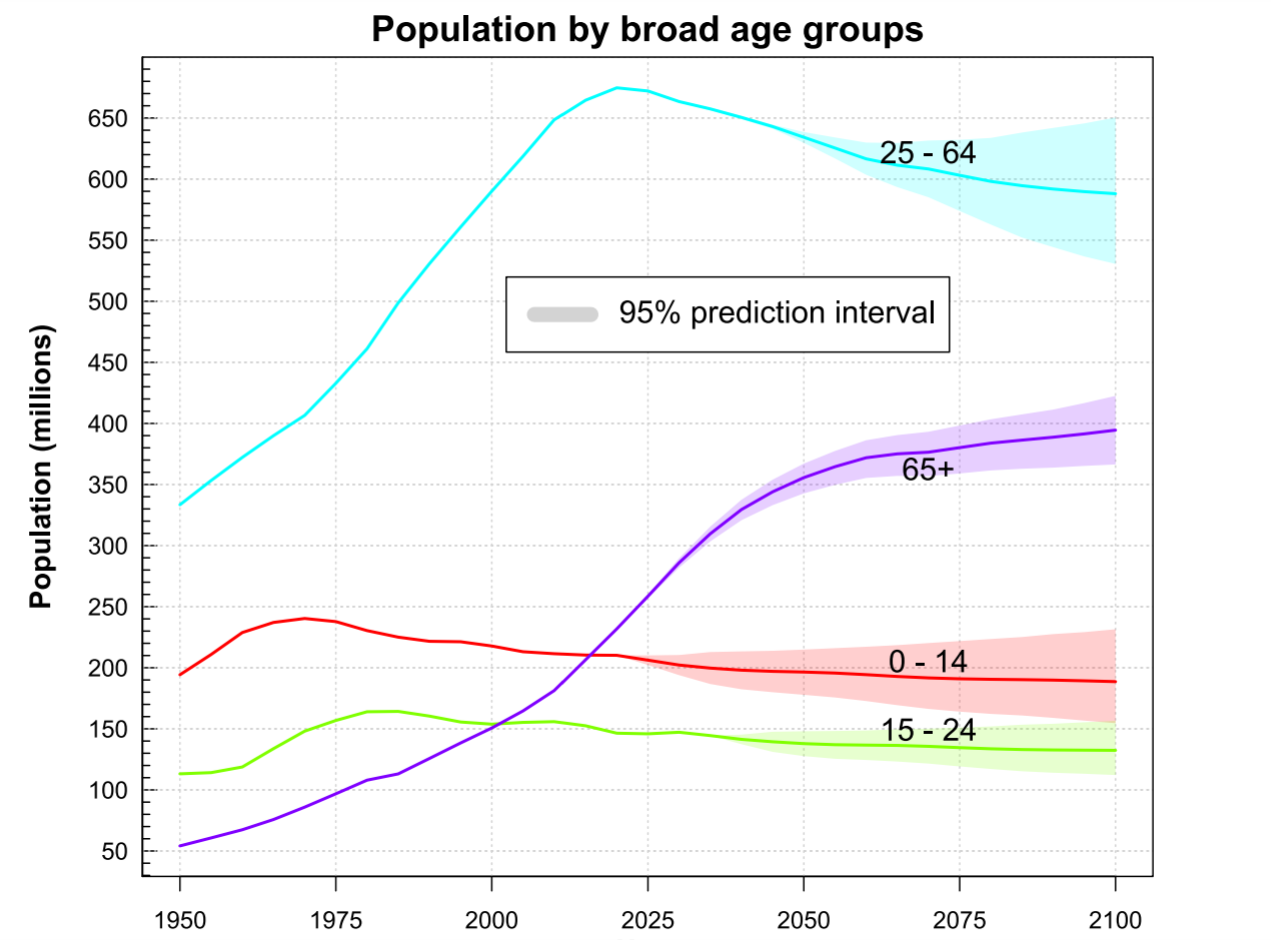
\includegraphics[width=0.8\textwidth]{figsrc/ch01/high_income_population_by_age_groups.png}
    \caption{高收入國家之年齡組別人口成長預測圖\cite{nations2019world}}
    \label{fig:population_age_world}
\end{figure}

\begin{figure}[htbp]
    \centering
    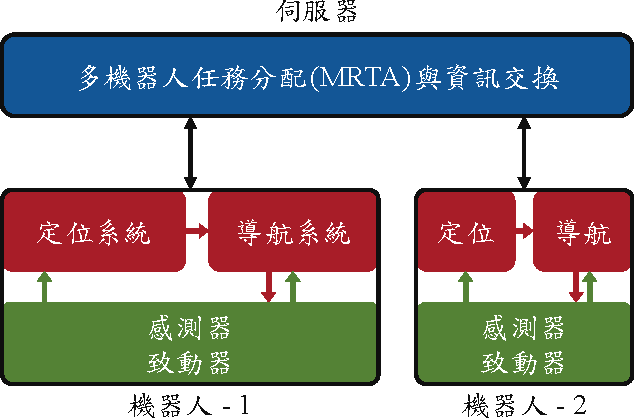
\includegraphics{figsrc/ch01/mrs_framework_zh.pdf}
    \caption{多機器人系統架構圖}
    \label{fig:mrs_framework}
\end{figure}

\begin{figure}[htbp]
    \centering
    \includesvg[width=0.9\textwidth]{figsrc/ch01/taiwan_population.svg}
    \caption{三階段年齡人口變動趨勢\cite{國發會年齡人口變動趨勢}}
    \label{fig:population_age_taiwan}
\end{figure}

有時候需要將圖片並排,可以參考以下的說明,其中建立兩個subfigure,其總大小需要稍微比頁面寬度略小不然會超出去(若真的要超出去可以參考下方註解,但盡量不要,會破壞排版,也可以將整個圖/表轉90度,參考\cref{c:appendix_caption}),故這邊設定單個子圖為0.48倍的頁面寬度,讓兩張圖一樣寬,有需要的話也可以自行調整兩者比例,$\backslash$hfill的目的是在兩張圖中間填充需要的空白,如果你的圖真的塞得有點極限也可以拿掉看看會不會就塞得進去。另外圖名(或是所有用到caption的地方),$\backslash$caption[顯示於目錄的標題]{顯示於內文的標題}可自由使用,若有些資訊或是備註不想讓他在目錄出現,可以弄一個比較簡短的。

\begin{figure}[htbp]
    \centering
    \begin{subfigure}[b]{0.48\textwidth}
        \centering
        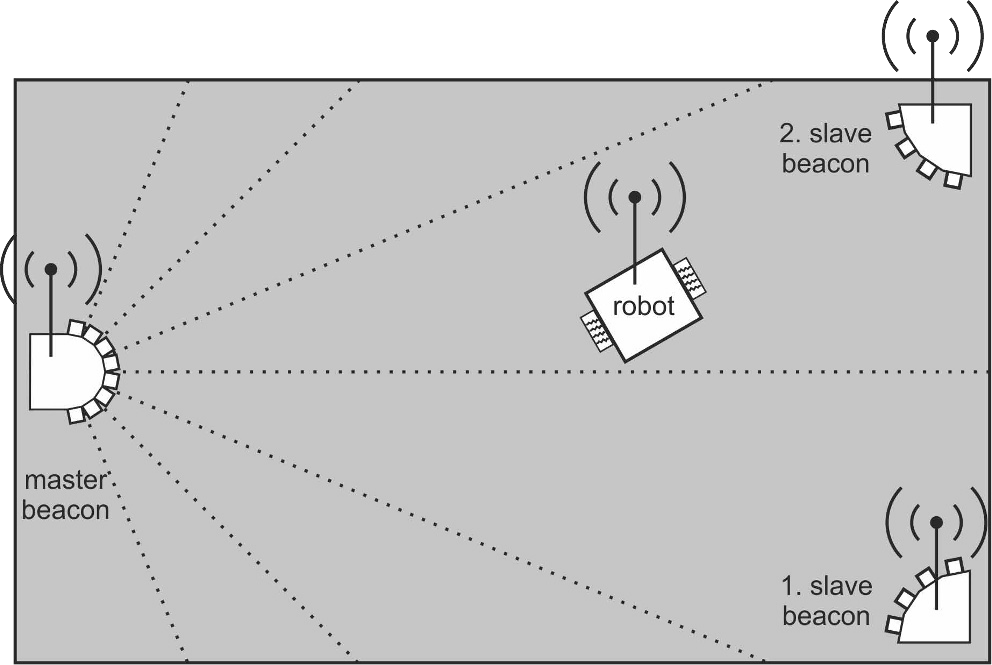
\includegraphics[width=\textwidth]{figsrc/ch01/eurobot_2012_ultrasonic_300dpi.png}
        \caption{超聲波定位系統示意圖\cite{eurobot_ultrasound_2013}}
        \label{fig:eurobot_2013_ultrasound}
    \end{subfigure}
    \hfill
    \begin{subfigure}[b]{0.48\textwidth}
        \centering
        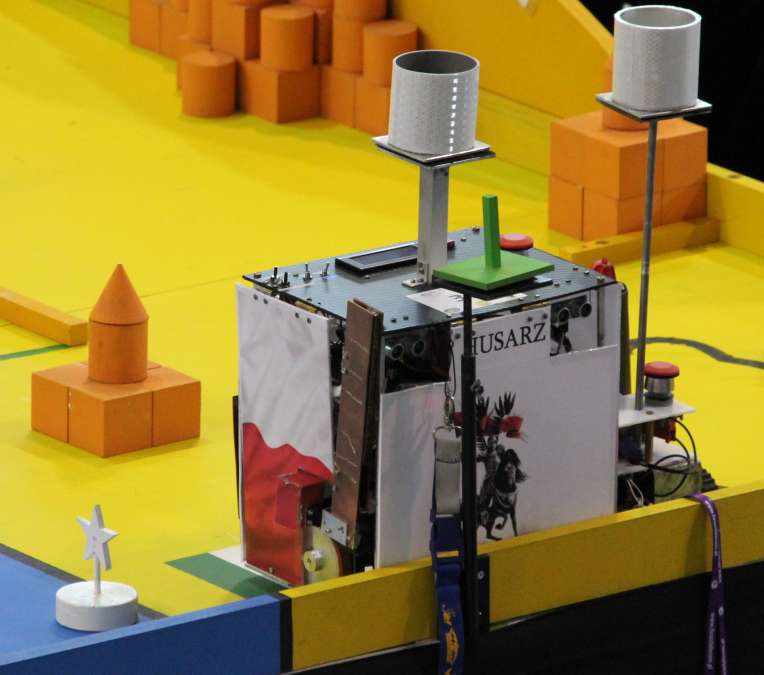
\includegraphics[width=\textwidth]{figsrc/ch01/eurobot_ros_2016_300dpi.png}
        \caption{SKaNeR所製作的機器人\cite{eurobot_ros_2016}}
        \label{fig:eurobot_ros_2016}
    \end{subfigure}
    \caption[隊伍於比賽時使用之系統示意圖與比賽實景(顯示於目錄的標題)]{隊伍於比賽時使用之系統示意圖與比賽實景(顯示於內文的標題)}
    \label{fig:eurobot_2013_2016}
\end{figure}

% 真的塞不下可考慮此方法,但需要依照情況微調
% \begin{figure}[htbp]
%     % figure is too large -> \centerline
%     \centerline{
%         \includegraphics[width=1.15\textwidth]{figsrc/ch04/sim_movement/eurobot_2022_0y1p_2.pdf}
%     }
%     \caption[模擬一:困難-2場景中三個演算法的導航結果]{模擬一:困難-2場景中三個演算法的導航結果(由左至右分別為APF、TEB及DWA的導航結果)}
%     \label{fig:sim_1_hard_2_movement}
% \end{figure}

\section{表格}
\label{sec:table}

表格通常會借助線上表格工具產生latex code後再貼入,筆者是使用\url{https://www.tablesgenerator.com/latex_tables}編輯後貼入,範例如\cref{table:exp_size}所示,而若需要整頁的表格請參考\cref{table:sim_1_result_sr_subopt_ta}。

\begin{table}[htbp]
\caption{實驗場域規格}
\label{table:exp_size}
\setlength{\tabcolsep}{7mm}
\begin{tabular}{lccc}
\hline
                           &    & 模擬環境  & 實驗環境  \\ \hline
\multirow{2}{*}{場地尺寸}      & 長  & 3m    & 4m    \\
                           & 寬  & 2m    & 2.3m  \\ \hline
\multirow{3}{*}{車輛尺寸}      & 長  & 0.2m  & 0.4m  \\
                           & 寬  & 0.2m  & 0.4m  \\
                           & 高  & 0.4m  & 0.3m  \\ \hline
\multirow{2}{*}{Beacon 尺寸} & 半徑 & 0.05m & 0.08m \\
                           & 高  & 0.51m & 0.29m \\ \hline
\end{tabular}
\end{table}

\section{方程式}
\label{sec:equation}

Latex語法用於打方程式應該是大家最熟悉的了,一樣有許多線上工具可以讓你打得更快,筆者這邊是使用\url{https://latex.codecogs.com/eqneditor/editor.php}協助產生一些少用的指令。也可以參考overleaf的官方文件:\url{https://www.overleaf.com/learn/latex/Mathematical_expressions},裡面有詳細說明這邊就不贅述,最簡單的就是用$a+b=c$這樣,以下是節錄自筆者論文內的方程式,使用align並且在thesis.tex中有設定可讓多個方程式跨頁方便排版。額外補充,\url{https://hackmd.io/@CynthiaChuang/Basic-LaTeX-Commands}這裡有人整理了常用數學符號指令。

\begin{align}
    \label{eqn:predict_mu_tf_zero}
	f(\boldsymbol{u}_{t},\boldsymbol{x}_{t}) &=
    \begin{bmatrix}
        v_{t}cos\theta\triangle t\\ 
        v_{t}sin\theta\triangle t\\ 
        0    \end{bmatrix}\\
    \label{eqn:predict_G_mat_zero}
    \boldsymbol{G}_t &= \begin{bmatrix}
    1 & 0 & -v_{t}sin\theta\triangle t\\
    0 & 1 & -v_{t}cos\theta\triangle t\\
    0 & 0 & 1 \end{bmatrix}\\
    \label{eqn:predict_V_mat_zero}
    \boldsymbol{V}_t &= \begin{bmatrix}
    cos\theta\triangle t & 0 \\    
    sin\theta\triangle t & 0 \\
    0 & 0 \end{bmatrix}\\
    \label{eqn:motion_noise_zero}
    \boldsymbol{M}_t &= \begin{bmatrix}
    \alpha_1 v_t^2 + \alpha_2\omega_t^2 & 0\\
    0 & \alpha_3 v_t^2 + \alpha_4\omega_t^2\\
    \end{bmatrix}
\end{align}

\section{演算法}
\label{sec:algorithm}

演算法也是有百百種用法,這邊使用的如下方所示,在thesis.tex 38行引用algorithm2e package,其餘請自行舉一反三XD。值得留意的是,有些老師會要求只有變數才能是斜體,若在演算法中要打方程式,要留意正體與斜體之間的差異,可以不要寫在方程式內(如下方calculate及return),或是使用$\backslash$text{}將文字括起來。

\begin{algorithm}[htbp]
\caption{EKF Localization: Predict Step}
\label{algo:ekf_predict}
\KwIn{$\boldsymbol{\mu}_{t-1}, \boldsymbol{\Sigma}_{t-1}, \boldsymbol{u}_{t}$}
\KwOut{$\boldsymbol{\bar{\mu}}_t, \boldsymbol{\bar{\Sigma}}_t$}
\BlankLine
calculate $f(\boldsymbol{u}_{t},\boldsymbol{x}_{t}), \boldsymbol{G}_t, \boldsymbol{V}_t, \boldsymbol{M}_t$\;
$\boldsymbol{\bar{\mu}}_t = \boldsymbol{\mu}_{t-1} + f(\boldsymbol{u}_{t},\boldsymbol{x}_{t})$\;
$\boldsymbol{\bar{\Sigma}}_t = \boldsymbol{G}_t \boldsymbol{\Sigma}_{t-1} \boldsymbol{G}_t^T + \boldsymbol{V}_t \boldsymbol{M}_t \boldsymbol{V}_t^T$\;
return $\boldsymbol{\bar{\mu}}_t, \boldsymbol{\bar{\Sigma}}_t$
\end{algorithm}

\section{列舉}
\label{sec:enumerate}

有時候會需要列舉的功能,原先的列舉每個標號之間空白太多,因此加上了[nosep],指令如下:

\begin{enumerate}[nosep]
\item 第一點
\item 第二點
\item 第三點
\end{enumerate}

\section{引用}
\label{sec:reference}

\subsection{文獻引用}

引用部分使用的是cite package,相關設定在thesis.tex 209-215行,目前設定為IEEEtran\_rchen的樣式,也就是依照動機系ICMEMS實驗室的論文模板魔改出來的特殊格式,若其他實驗室想使用此模板,建議將thesis.tex 210行改為IEEEtran格式並刪除暫存檔後重新編譯。所有文獻皆以BibLaTeX格式記錄在thesis.bib中(目前裡面是筆者的引用資料,提供給大家參考),可以使用google學術搜尋找到想引用的論文後,按cite找到他的BibLaTeX格式並複製貼上到thesis.bib中。

若是ICMEMS的實驗室同學請特別留意:
\begin{enumerate}[nosep]
\item @inproceedings(研討會論文),老師要求要有舉辦地點與詳細時間,因此可參考thesis.bib中的寫法補上address,範例如下:address={Bangkok, Thailand, December 14 - 17}。
\item @online(線上資料),此格式如\cite{eurobot}所示,請自行參閱thesis.bib中內容。
\item @emptymisc(空白的格式),若喬不好格式可用這個,完全自己打的reference,尤其是當要引用中文文獻時,避免全/半形標點符號混用,範例請見thesis.bib。
\end{enumerate}


以下範例擷取自筆者碩士論文中緒論的第一節:

隨著電子商務的蓬勃發展,物流與配送需求逐年上升。如在工廠內的揀貨,基本為勞力較為密集的產業。而隨著勞力成本提高,且業者越來越不容易找到願意從事此類單調生產工作的勞動人力,因此,應用於物流配送之自動化技術已成為顯學,如此不只能減緩缺工問題,也能提升貨品搬運效率、運送穩定度以及降低生產成本。

此外,根據聯合國經濟和社會事務部在2019年發布世界人口展望報告(World Population Prospects 2019)\cite{nations2019world}指出,儘管全球人口仍在增長,但部分國家的總人口正在減少。以高收入國家的人口預測圖為例(\cref{fig:population_age_world}),可以發現25至64歲的青壯年勞動力逐年降低,且老年人口也逐年增加。同時在中華民國科技部人文及社會科學研究發展司的報告中也指出\cite{人文與社科簡訊_人口老化},預期將於2022年後台灣開始進入人口負成長時期,且人口也逐漸老化(\cref{fig:population_age_taiwan}),更直接對勞動力產生衝擊。

自嚴重特殊傳染性肺炎(COVID-19)爆發以來,世界各國實施大規模封鎖令,希望降低人們接觸的機率,導致大部分的勞動力無法進入市場服務。同時,冒著風險維持必要物資運送的人員,也籠罩在染疫的巨大風險之中;舉凡航運業、製造業甚至外送業及服務業都面臨嚴峻的缺工問題。由此可見,引進機器替代勞力有其必要性與急迫性,相較於人力來說,由機器執行重複性高的工作時,可得更精準、穩定且高效率的成果,也能在疫情期間降低人們因接觸產生的染疫風險。

2013年BURKODI等人\cite{eurobot_ultrasound_2013}總結了其隊伍:SKaNeR,於Eurobot 2012賽事中的結果,該隊伍放置超聲波模組於\cref{fig:eurobot_2013_2016}~(a)中三個Beacon處,並
利用超聲波向場地內掃描,找出場上所有機器人的位置(如\cref{fig:eurobot_2013_2016}~(a)所示)。2016年Granosik等人\cite{eurobot_ros_2016}利用機器人作業系統(Robot Operating System,後稱ROS)\cite{ros_2009}中的導航框架(Navigation Stack),搭配SLAM於Eurobot 2016的場地內進行定位與導航(如\cref{fig:eurobot_2013_2016}~(b)所示)。


\subsection{素材引用}

為了提供高度客製化的內文素材引用格式(迎合老師的奇怪規範),除了文獻以外的引用,在本範例文件中皆使用cleveref這個套件,在thesis.tex的48-57行筆者依照動機系ICMEMS實驗室的論文規範客製化了chapter、section、subsection、subsubsection、figure、table、equation、algorithm及appendix的格式,其文中引用結果如下所示:

引用章:\cref{c:introduction}、引用節:\cref{sec:architecture}、引用小節:\cref{subsec:subsection}、引用圖片:\cref{fig:population_age_world}、引用表格:\cref{table:exp_size}、引用方程式:\cref{eqn:predict_mu_tf_zero}、引用演算法:\cref{algo:ekf_predict}、引用附錄:\cref{c:appendix_caption}。
% \input{02_problem_formulation}
% \input{03_robot_localization_and_tracking}
% \input{04_multi_robot_navigation}
% \input{05_system_implement_and_result}
% \input{06_conclusion}

% do not use the hyphen in bibliography
\tolerance=1
\emergencystretch=\maxdimen
\hyphenpenalty=10000
\hbadness=10000
\renewcommand{\bibname}{\Large\bfseries\centering{參考文獻}\vspace{10pt}}
\cleardoublepage
% \phantomsection % for hyperref to correct the link
\addcontentsline{toc}{chapter}{參考文獻}
\bibliographystyle{IEEEtran_rchen}

% Your bibliography goes here
{\singlespacing
 \bibliography{thesis}
}

% \appendix
\titlecontents{chapter}% <section-type>
  [0pt]% <left>
  {}% <above-code>
  {\bfseries 附錄\thecontentslabel \quad}% <numbered-entry-format>
  {\bfseries}% <numberless-entry-format>
  {\bfseries\hfill\contentspage}% <filler-page-format>
\appendix

\titleformat{\chapter}
  {\Large\bfseries\centering}
  {附錄\,\thechapter}{1em}{\Large}
  
\chapter{附錄說明}
\label{c:appendix_caption}

此處為附錄,若有需要放置一些必要資訊,但又不想放在內文裡面,可以放在這邊。11行以前的東西不要刪掉,是為了定義附錄的格式,在此處每新增一個chapter就會由附錄A開始編號至附錄B等以此類推,我是因為圖表過大因此放在附錄,\cref{table:sim_1_result_sr_subopt_ta}為跨頁表格的範例,基本上與一般表格相同,只是最外面改為sidewaytable而已,若是要使用跨頁圖,則是使用sidewayfigure即可。

\begin{sidewaystable}[htbp]
\caption{模擬一:不同場景內三種演算法的導航成功率(SR)、次優性與到達時間(TA)之統計量}
\label{table:sim_1_result_sr_subopt_ta}
\begin{tabular}{ccccccccccc}
\hline
\multicolumn{1}{l}{}  & \multicolumn{1}{l}{} & \multicolumn{3}{c}{APF}                      & \multicolumn{3}{c}{TEB}                      & \multicolumn{3}{c}{DWA}                      \\ \cmidrule(r){3-5} \cmidrule(r){6-8} \cmidrule(r){9-11}
\multicolumn{1}{l}{}  & \multicolumn{1}{l}{} & SR(\%) & 次優性(\%) & \multicolumn{1}{c}{TA(s)} & SR(\%) & 次優性(\%) & \multicolumn{1}{c}{TA(s)} & SR(\%) & 次優性(\%) & \multicolumn{1}{c}{TA(s)} \\ \hline
\multirow{2}{*}{簡單-1} & 平均值$^\dagger$          & 100.00 & -1.50   & 5.72                      & 100.00 & 0.37    & 5.87                      & 100.00 & -2.48   & 7.83                      \\
                      & 標準差                  &        & 0.30    & 0.03                      &        & 0.28    & 0.04                      &        & 0.15    & 0.62                      \\
\multirow{2}{*}{簡單-2} & 平均值                  & 100.00 & -0.58   & 7.83                      & 100.00 & -0.37   & 6.32                      & 96.67  & 3.28    & 20.31                     \\
                      & 標準差                  &        & 0.31    & 0.07                      &        & 0.25    & 0.06                      &        & 5.32    & 6.79                      \\
\multirow{2}{*}{簡單-3} & 平均值                  & 100.00 & -2.41   & 7.67                      & 100.00 & -1.51   & 6.24                      & 100.00 & -2.88   & 13.60                     \\
                      & 標準差                  &        & 0.49    & 0.06                      &        & 0.24    & 0.06                      &        & 3.88    & 3.76                      \\ \hline
\multirow{2}{*}{中等-1} & 平均值                  & 100.00 & -1.07   & 11.07                     & 100.00 & -2.08   & 9.58                      & 56.67  & -2.35   & 25.07                     \\
                      & 標準差                  &        & 0.60    & 0.17                      &        & 4.27    & 0.93                      &        & 7.46    & 4.91                      \\
\multirow{2}{*}{中等-2} & 平均值                  & 100.00 & 1.28    & 10.52                     & 100.00 & -2.66   & 8.87                      & 23.33  & -1.70   & 29.18                     \\
                      & 標準差                  &        & 1.43    & 0.10                      &        & 0.27    & 0.08                      &        & 3.06    & 11.48                     \\
\multirow{2}{*}{中等-3} & 平均值                  & 100.00 & -0.54   & 10.94                     & 100.00 & -2.11   & 9.83                      & 16.67  & -7.65   & 21.16                     \\
                      & 標準差                  &        & 0.87    & 0.17                      &        & 5.66    & 0.93                      &        & 2.70    & 7.09                      \\ \hline
\multirow{2}{*}{困難-1} & 平均值                  & 100.00 & -0.05   & 10.39                     & 60.00  & 17.02   & 13.46                     & 0.00   & NaN$^\ddagger$     & \multicolumn{1}{r}{NaN}   \\
                      & 標準差                  &        & 0.35    & 0.33                      &        & 11.89   & 3.44                      &        & NaN     & \multicolumn{1}{r}{NaN}   \\
\multirow{2}{*}{困難-2} & 平均值                  & 100.00 & -0.22   & 10.21                     & 96.67  & 0.68    & 9.41                      & 3.33   & 26.46   & 39.34                     \\
                      & 標準差                  &        & 0.58    & 0.25                      &        & 5.00    & 1.01                      &        & NaN     & \multicolumn{1}{r}{NaN}   \\
\multirow{2}{*}{困難-3} & 平均值                  & 100.00 & 0.22    & 9.53                      & 100.00 & -1.91   & 8.72                      & 0.00   & NaN     & \multicolumn{1}{r}{NaN}   \\
                      & 標準差                  &        & 0.31    & 0.10                      &        & 0.51    & 0.13                      &        & NaN     & \multicolumn{1}{r}{NaN}   \\ \hline
\multicolumn{11}{l}{$^\dagger$~平均值與標準差皆使用樣本平均值與樣本標準差進行估計}\\
\multicolumn{11}{l}{$^\ddagger$~ NaN表示在該場景的三十組導航結果中,因成功率過低導致無法計算平均值/標準差。}
\end{tabular}
\end{sidewaystable}

\end{document}
